\documentclass[10pt]{beamer}

\usetheme{default} % theme général du diaporama

% paquets pour le français
\usepackage[T1]{fontenc}
\usepackage[utf8]{inputenc}
\usepackage{graphicx}

% use serif font with rm
% \renewcommand{\familydefault}{\rmdefault}

\title{Identification spatiale continue des points chauds de diversité beta à l'aide de modèles de distribution d'espèces}
\author{Gabriel Dansereau}

\begin{document}

\begin{frame}
  \titlepage
\end{frame}

\begin{frame}
  \frametitle{Plan de la présentation}
  \begin{itemize}
    \item Objectif
    \item Description eBird
    \item Données BIOCLIM
    \item Données brutes
    \begin{itemize}
      \item Méthode présence-absence
      \item Résultats
    \end{itemize}
    \item Modèles de distribution d'espèces (SDM)
    \begin{itemize}
      \item Méthode BIOCLIM
      \item Résultats
    \end{itemize}
    \item À venir
    \item Autres points
  \end{itemize}
\end{frame}

\begin{frame}
  \frametitle{Objectif}
  \begin{itemize}
    \item Objectif général: Identification des zones qui contribuent le plus à la diversité beta dans l'espace
    \begin{itemize}
      \item Échelle continue, étendue
      \item Diversité beta: composition spécifique, interactions
      \item Prévision changements climatiques
      \item Données science ouverte \& science citoyenne
    \end{itemize}
    \medskip
    \item 1ère partie: Test de la méthode
    \begin{itemize}
      \item LCBD sur données brutes
      \item Développement méthode SDM
      \item LCBD sur sorties SDM
      \item Scénarios changements climatiques IPCC
    \end{itemize}
    \medskip
    \item 2e partie: Applications aux interactions
  \end{itemize}
\end{frame}

\begin{frame}
  \frametitle{Description eBird}
  \begin{itemize}
    \item Parulines - Famille Parulidae
    \item CA, US, MX
    \item 23 000 000 observations (uniques)
    \item 63 espèces: quartiles = 2, 11 000, 140 000, 370 000, 4 000 000
    \item Années: quartiles = 1838, 2012, 2015, 2018, 2019
  \end{itemize}
\end{frame}

\begin{frame}
  \frametitle{Données brutes - Méthodes}
  Presence-absence par espèce
  \begin{itemize}
    \item Pixels - Résolution 5 arc-minutes
    \item Matrice 661 x 1141 (env. 750 000 pixels)
    \item 100 000 sites avec observations sur 400 000 sites
  \end{itemize}
  \medskip
  Matrice Y sites x espèces
  \begin{itemize}
    \item 100 000 x 63
    \item Transformation Hellinger
  \end{itemize}
  \medskip
  Calcul LCBD
  \begin{itemize}
    \item Var(Y), SStotal, BDtotal, SSi, LCBDi...
    \item Test permutation (correction?)
  \end{itemize}
\end{frame}

\begin{frame}
  \frametitle{Données brutes - 1 espèce, beaucoup d'observations}
  \begin{figure}
    \centering
    \hspace*{-0cm}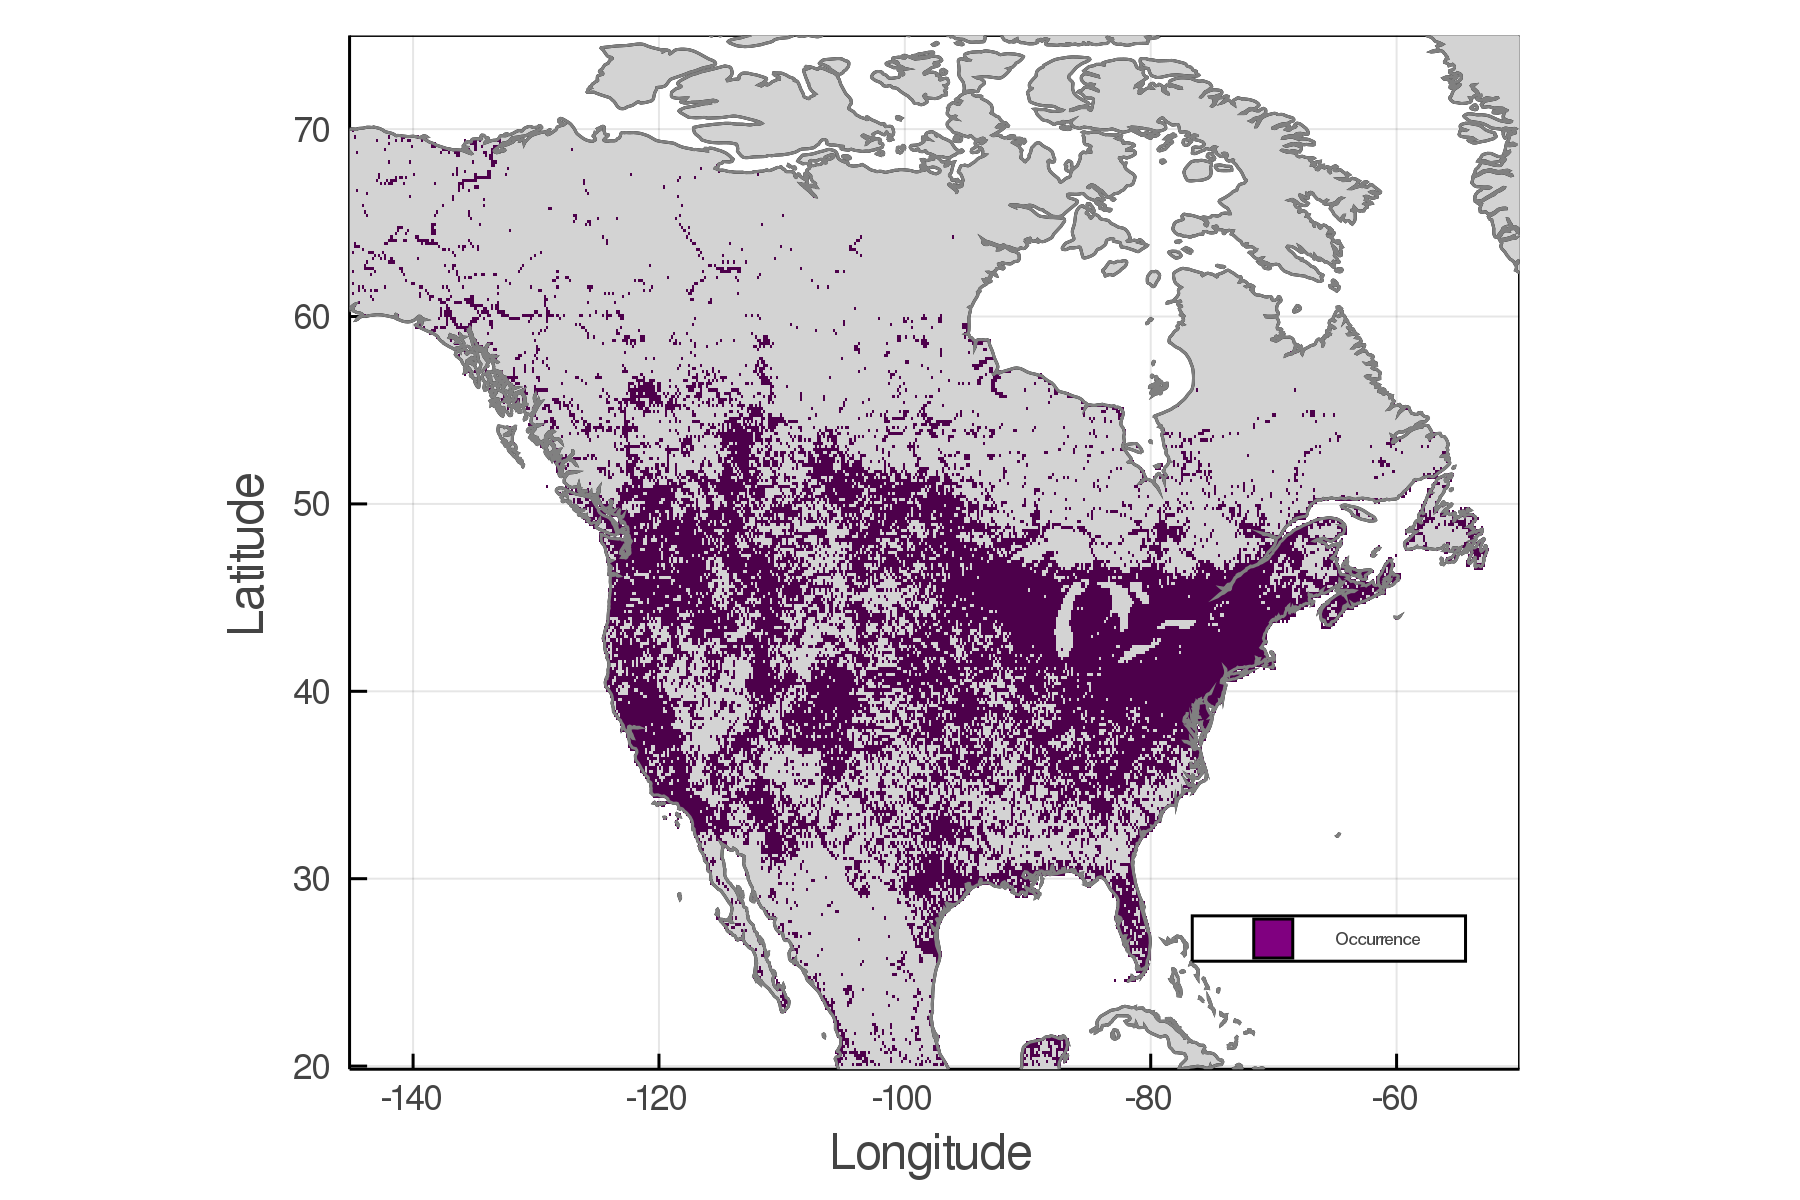
\includegraphics[scale=0.17]{fig/01_raw_singlesp.png}
    \caption{Distribution des observations de la Paruline jaune (présence-absence)}
  \end{figure}
\end{frame}

\begin{frame}
  \frametitle{SDM - 1 espèce, beaucoup d'observations}
  \begin{figure}
    \centering
    \hspace*{-0cm}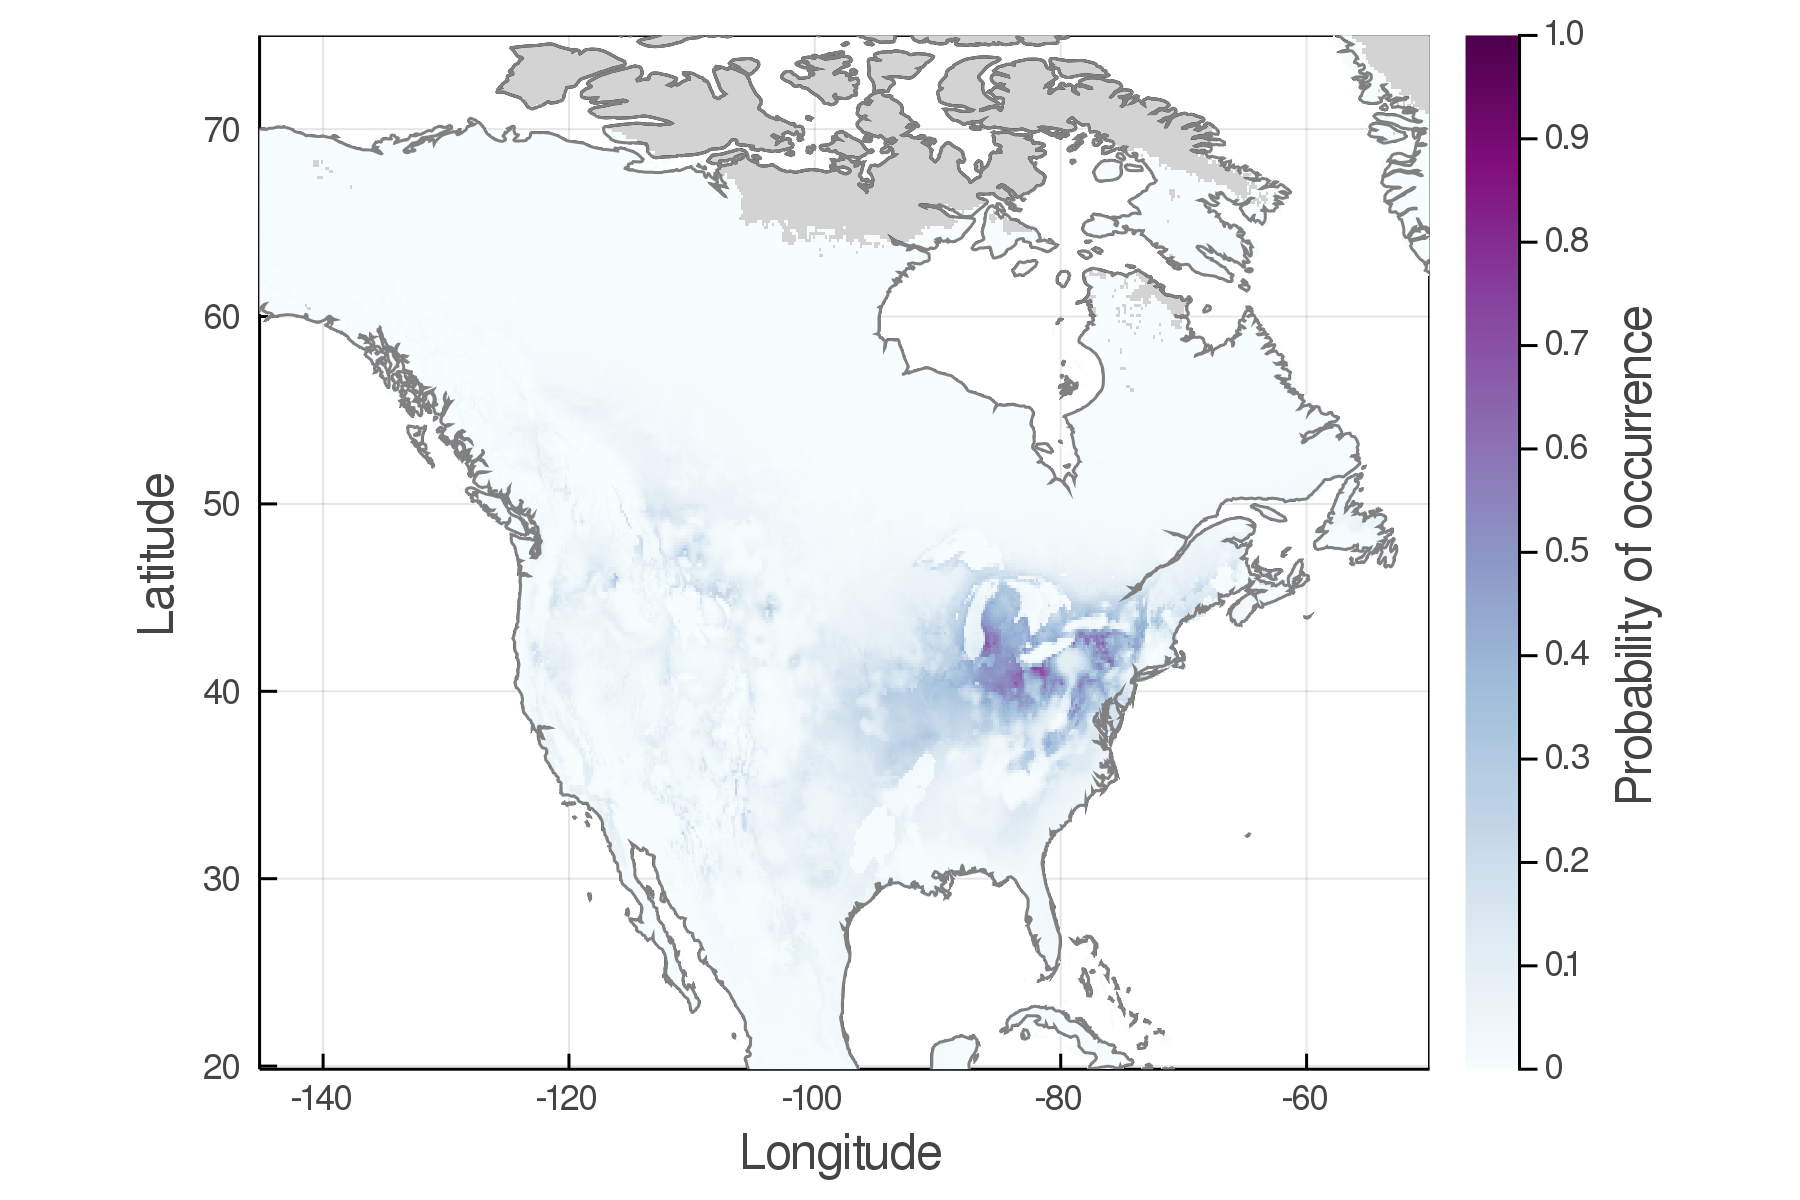
\includegraphics[scale=0.17]{fig/01_sdm_singlesp.png}
    \caption{Sortie du SDM pour la Paruline jaune}
  \end{figure}
\end{frame}

\begin{frame}
  \frametitle{Données brutes - Richesse spécifique (nombre d'espèces)}
  \begin{figure}
    \centering
    \hspace*{-0cm}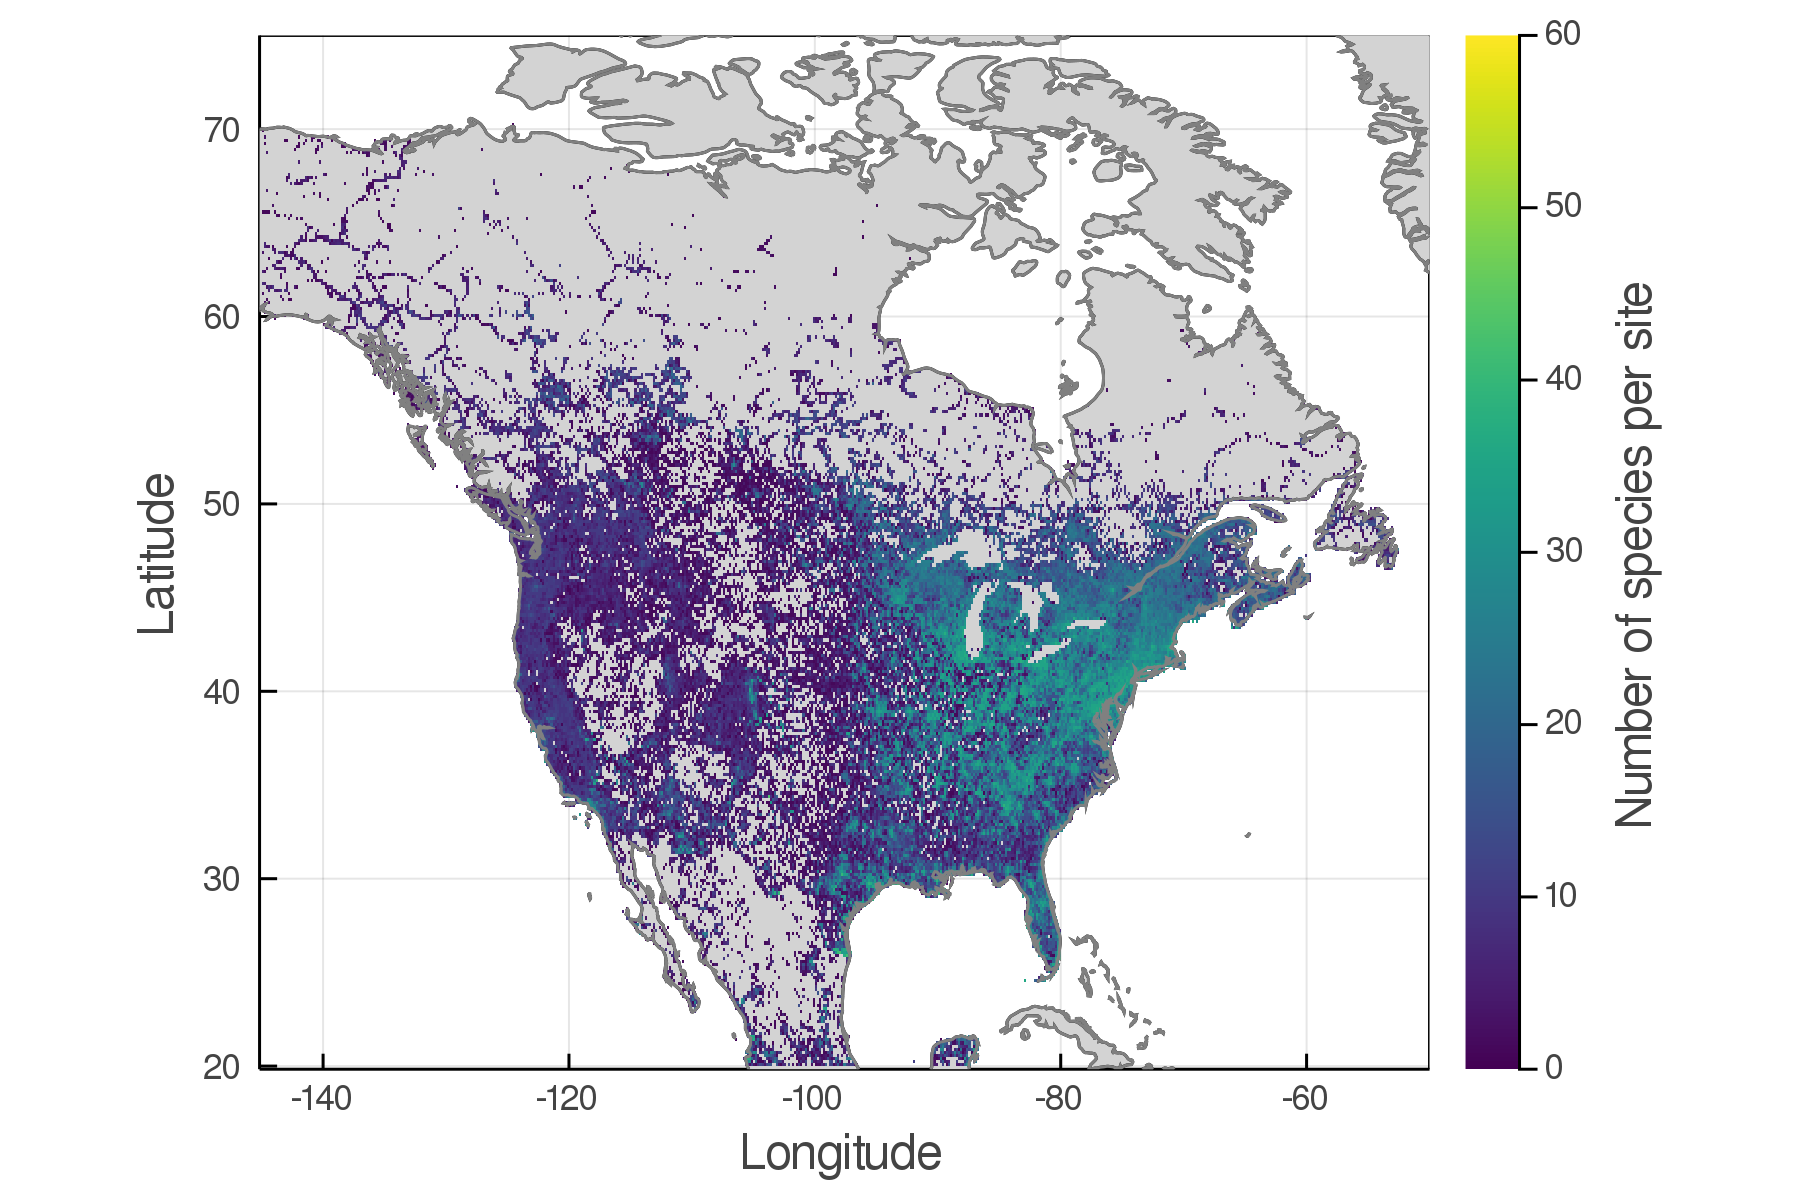
\includegraphics[scale=0.17]{fig/03_raw_richness.png}
  \end{figure}
\end{frame}

\begin{frame}
  \frametitle{SDM- Richesse spécifique (nombre d'espèces)}
  \begin{figure}
    \centering
    \hspace*{-0cm}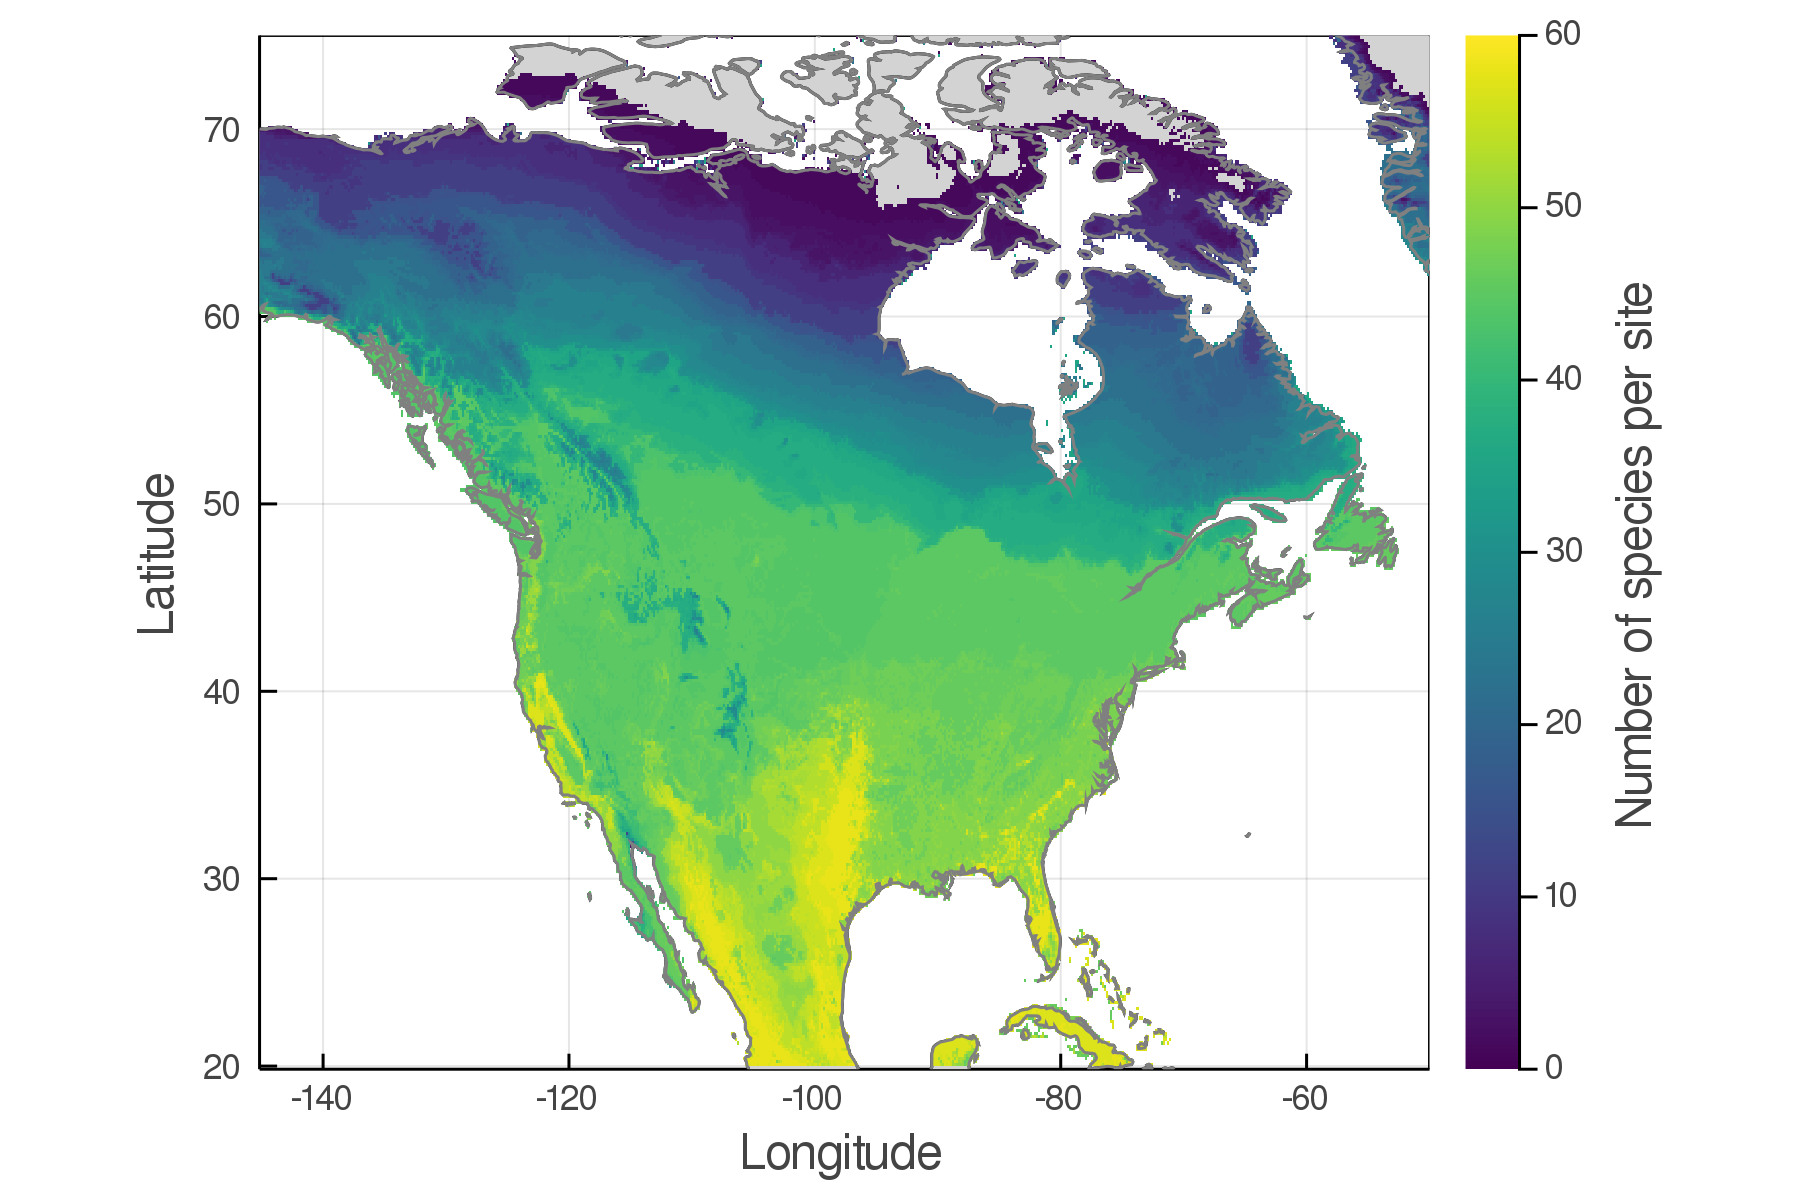
\includegraphics[scale=0.17]{fig/03_sdm_richness.png}
  \end{figure}
\end{frame}

\begin{frame}
  \frametitle{Données brutes- LCBD}
  \begin{figure}
    \centering
    \hspace*{-0cm}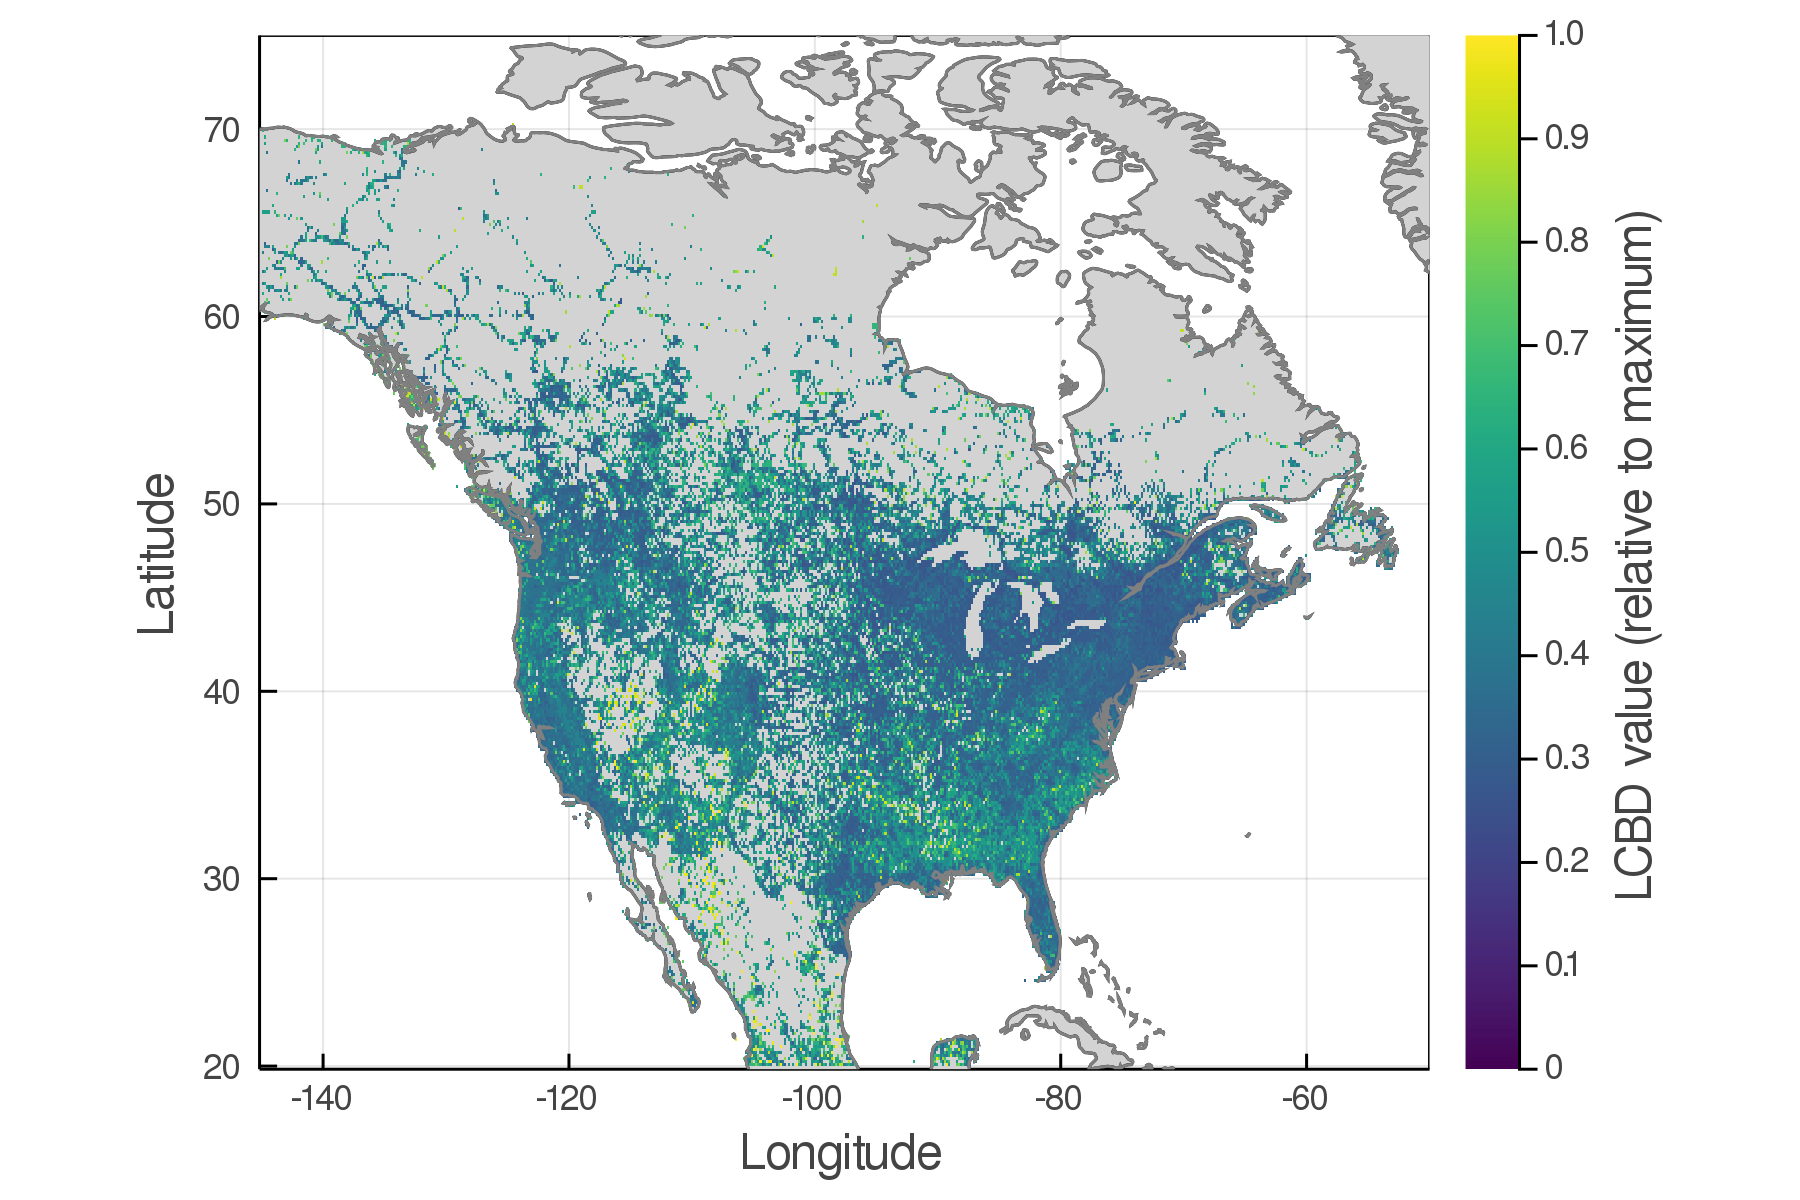
\includegraphics[scale=0.17]{fig/05_raw_lcbd-transf.png}
  \end{figure}
\end{frame}

\begin{frame}
  \frametitle{SDM - LCBD}
  \begin{figure}
    \centering
    \hspace*{-0cm}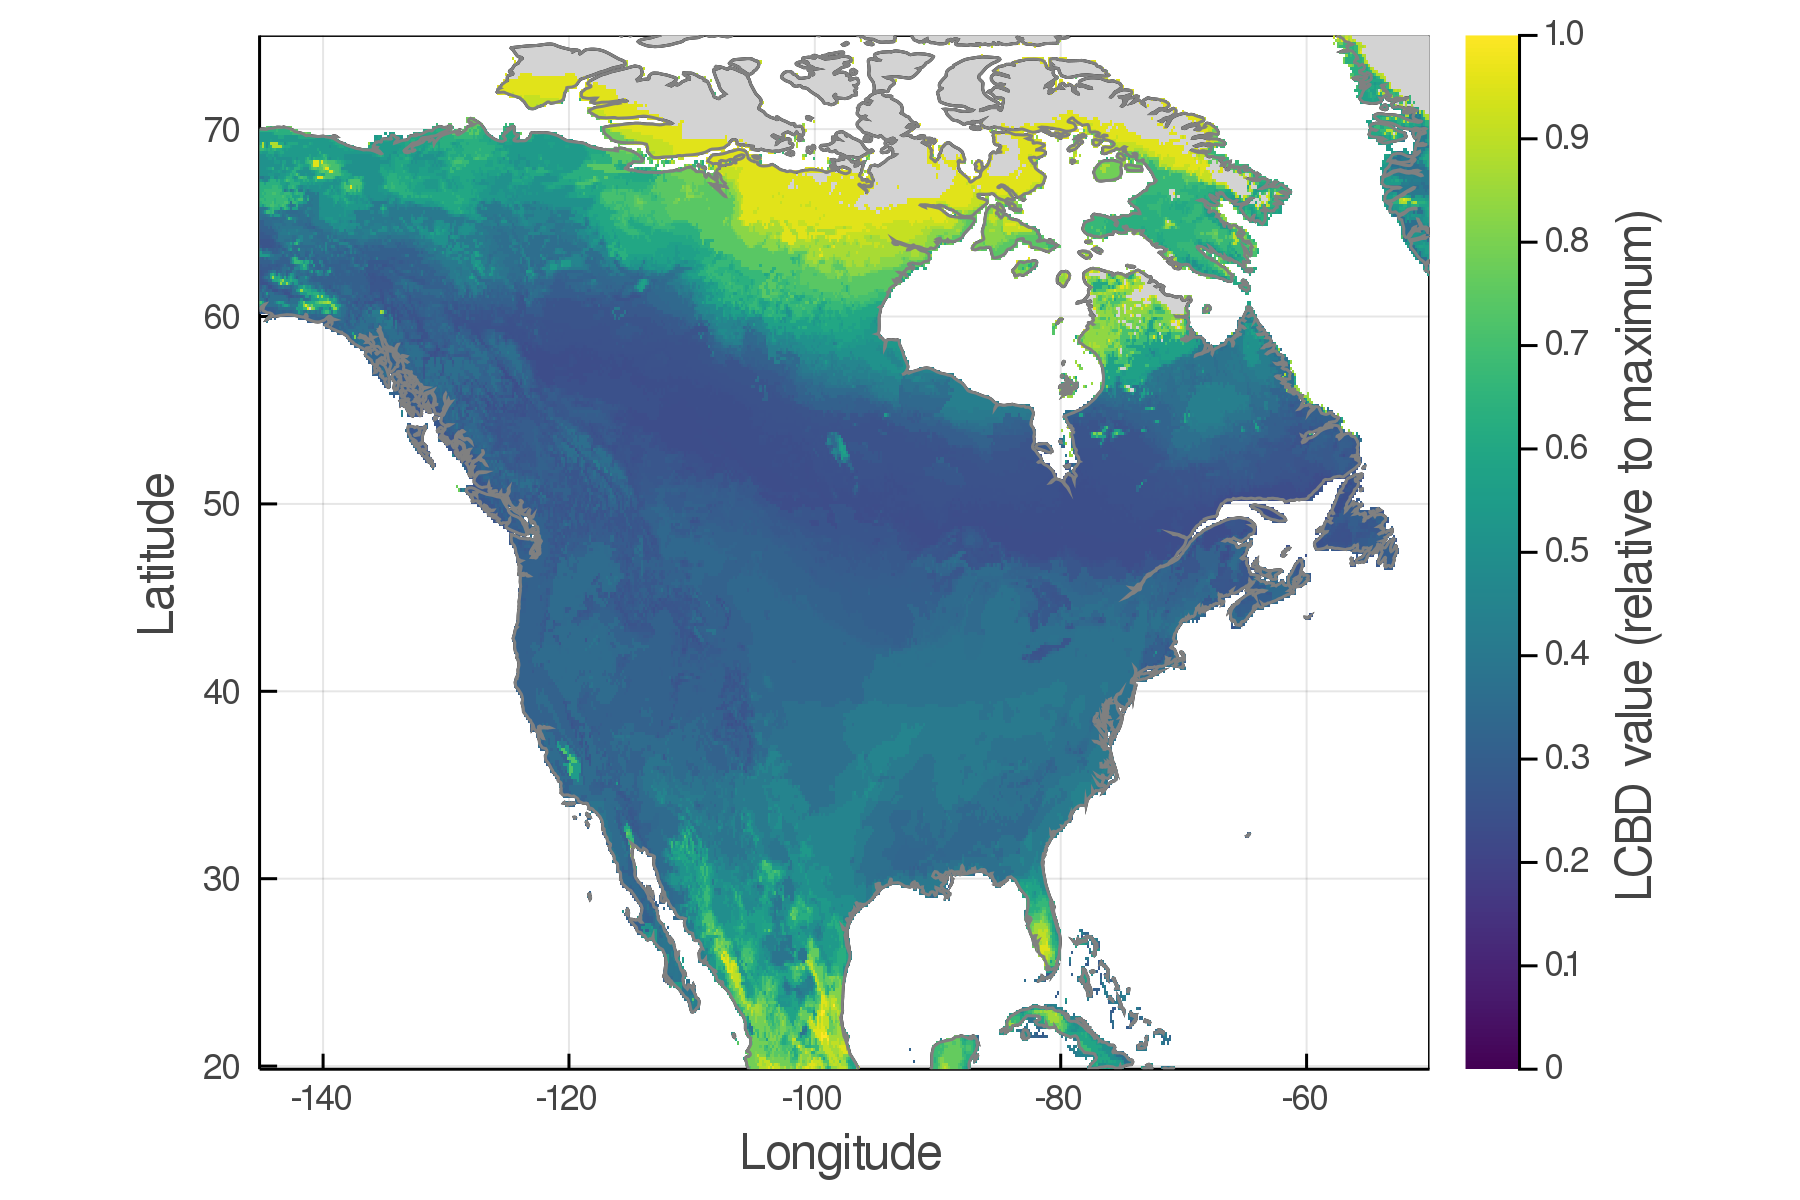
\includegraphics[scale=0.17]{fig/05_sdm_lcbd.png}
  \end{figure}
\end{frame}

\begin{frame}
  \frametitle{Données brutes - Relation LCBD-richesse}
  \begin{figure}
    \centering
    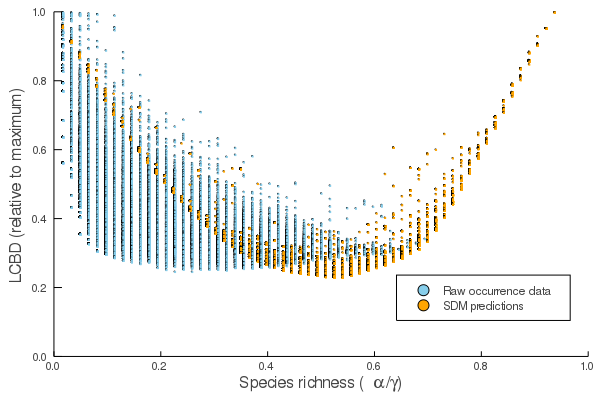
\includegraphics[scale=0.4]{fig/06_cmb_relation-oneplot.png}
  \end{figure}
\end{frame}

\end{document}
